\section{METODOLOGIA}
\subsection{Visão Geral}
A plataforma colcom se propõe a ser um ambiente de debates justo, transparente, participativo e deliberativo. O nome colcom é um acrônimo para “colaboração e competição", que são as principais formas de atuação na plataforma. A lógica de operação da plataforma pode ser sumarizada nos seguintes passos:

\begin{itemize}
    \item Um usuário incia um tópico;
    \item Usuários submetem \textit{posts} em reposta ao tópico;
    \item Usuários colaboram no aprimoramento de \textit{posts}, através de sugestões de edição e críticas das falhas encontradas;
    \item Usuários competem para que sua resposta seja a mais votada do tópico.
\end{itemize}

Além disso, a plataforma possibilita aos usuários avaliar a relevância percebida de cada conteúdo, seja ele um tópico, \textit{post} ou crítica, e também confere aos usuários a possibilidade de promoverem um tópico, aumentando assim a sua visibilidade no dia corrente. Optamos por permitir apenas a promoção de tópicos a fim de evitar efeitos de polarização, dado que são os tópicos que agregam todas as respostas dos usuários.




\subsection{Requisitos Funcionais}

Nesta seção serão descritos os requisitos funcionais da aplicação, que se referem às declarações de serviços que o sistema deve fornecer, especificando inclusive as condições sobre as quais devem ser fornecidos \cite{requirements}.

\subsubsection{[RF01] Cadastrar um usuário}
A aplicação deve possibilitar o cadastro de novos usuários por meio do fornecimento de um nome de usuário, e-mail e senha.

\subsubsection{[RF02] Efetuar o \textit{login} de um usuário}
A aplicação deve possibilitar que usuários previamente cadastrados consigam acessar sua conta ao fornecer seu nome de usuário ou e-mail e sua senha.

\subsubsection{[RF03] Avaliar um conteúdo como relevante ou não}
Usuários que estejam logados devem ser capazes de avaliar se um conteúdo como relevante ou não por meio de botões de voto.

\subsubsection{[RF04] Salvar um conteúdo}
Usuários que estejam logados devem ser capazes de salvar um conteúdo em sua coleção de favoritos.

\subsubsection{[RF05] Criar um tópico}
Usuários que estejam logados devem ser capazes de criar novos tópicos através de um botão. O botão ao ser acionado deve abrir uma caixa de diálogo para a inserção dos dados do tópico, que incluem: título, possibilidade de usuários submeterem múltiplas respostas, e as possíveis respostas, caso o tópico se trate de uma enquete.

\subsubsection{[RF06] Promover um tópico}
Usuários que estejam logados devem ser capazes de promover um tópico, i.e., conferir um voto de visibilidade para o tópico até o fim do dia corrente.

\subsubsection{[RF07] Visualizar tópicos registrados}
Todos os usuários devem ser capazes de visualizar os tópicos registrados, ordenados pelo número de promoções, ou data de criação.

\subsubsection{[RF08] Visualizar tópicos salvos}
Usuários que estejam logados devem ser capazes de visualizar os tópicos salvos anteriormente, ordenados pela data de salvamento.

\subsubsection{[RF09] Escrever corpo de um conteúdo}
A aplicação deve fornecer um editor de texto com várias funcionalidades e capacidades de estilização para viabilizar o uso da plataforma para diversos contextos diferentes.

\subsubsection{[RF10] Criar um \textit{post} em resposta a um tópico}
Usuários que estejam logados devem ser capazes de responder um dado tópico através da criação de um \textit{post}. Ao criar o \textit{post}, o usuário deve fornecer: um título, um corpo do \textit{post} e, caso o tópico seja uma enquete, uma opção de resposta.

\subsubsection{[RF11] Votar em um \textit{post}}
Usuários que estejam logados devem ser capazes de votar em um \textit{post} de um tópico para representar sua escolha.

\subsubsection{[RF12] Editar um \textit{post}}
O autor de um \textit{post} deve ser capaz de realizar edições em um \textit{post} e salvá-las, criando assim uma nova versão do \textit{post}. Uma mensagem contendo uma explicação das alterações deve ser fornecida pelo usuário.

\subsubsection{[RF13] Criar uma sugestão de edição para um \textit{post}}
Usuários logados que não sejam o autor de um \textit{post} devem ser capazes de submeter uma sugestão de alteração para o \textit{post}. Uma mensagem contendo uma explicação das alterações deve ser fornecida pelo usuário.

\subsubsection{[RF14] Criar um “ramo" de uma versão específica de um \textit{post}}
Usuários logados que não sejam o autor de um \textit{post} devem ser capazes de fazer uma \textit{branch} de um \textit{post} em qualquer versão, i.e., criar uma cópia do \textit{post} em que a autoria passa a ser do usuário solicitante.

\subsubsection{[RF15] Visualizar uma versão específica de um \textit{post}}
Usuários que estejam logados devem ser capazes de visualizar uma versão específica de um \textit{post} através da manipulação de uma linha do tempo que exiba todas versões da aplicação.

\subsubsection{[RF16] Visualizar proposições de edição de um \textit{post}}
O autor de um \textit{post} deve ser capaz de visualizar todas as proposições de edição feitas por outros usuários para este \textit{post}.

\subsubsection{[RF17] Acatar e rejeitar proposições de edição de um \textit{post}}
O autor de um \textit{post} deve ser capaz de rejeitar ou incorporar proposições, através de um \textit{merge}, em um \textit{post} de sua autoria.

\subsubsection{[RF18] Visualizar críticas de uma versão específica de um \textit{post}}
A aplicação deve possibilitar que todas as críticas contidas em cada trecho, de cada versão de um \textit{post}, sejam visualizáveis para todos os usuários da aplicação.

\subsubsection{[RF19] Realizar críticas em um \textit{post}}
Usuários que estejam logados devem ser capazes de criticar qualquer trecho de um \textit{post}, fornecendo um título e corpo para a crítica.



\subsection{Requisitos Não Funcionais}
Nesta sessão, estão descritos os requisitos não funcionais. Contrariamente aos requisitos funcionais, não há um consenso bem estabelecido sobre o que são, havendo diversas definições na literatura \cite{requirements, requirements2}. Aqui, usaremos a definição comum de que são requisitos que se referem a outros aspectos qualitativos que não funcionalidades em si. Para nosso projeto, separamos os requisitos não funcionais de acordo com os seguintes aspectos: usabilidade, desempenho, segurança, manutenibilidade, portabilidade e legalidade.

\subsubsection{Usabilidade}

\paragraph{[RNF01] Intuitividade}
A aplicação deve ter um design intuitivo, aproveitando-se de símbolos comumente já usados em redes sociais populares.

\paragraph{[RNF02] Responsividade}
A aplicação deverá ter uma boa adaptação à diferentes resoluções de tela, de modo que funcione bem em dispositivos móveis e em computadores pessoais.

\paragraph{[RNF03] Consistência}
A aplicação deve ter um design consistente, de modo que usuários possam inferir o funcionamento de outras partes da aplicação a partir do que já foi visto.


\subsubsection{Desempenho}

\paragraph{[RNF04] Usuários simultâneos}
A aplicação deve suportar o uso de mais de 100 usuários simultâneos.

\paragraph{[RNF05] Tempo de resposta}
A aplicação deve demorar não mais que 1 segundo para retornar uma resposta.


\subsubsection{Segurança}

\paragraph{[RNF06] Controle de acesso}
A aplicação deve garantir que somente usuários autorizados publiquem e editem conteúdos.

\paragraph{[RNF07] Obfuscação de dados sensíveis}
A aplicação deve criptografar os dados sensíveis a serem armazenados.


\subsubsection{Manutenibilidade}

\paragraph{[RNF08] SCV}
O código fonte deve ser escrito fazendo-se uso de um SCV para registar as alterações realizadas.

\paragraph{[RNF09] Código aberto}
O código fonte deve ser disponibilizado gratuitamente na plataforma \textit{GitHub}.


\subsubsection{Portabilidade}

\paragraph{[RNF10] \textit{Self-hosting}}
A aplicação deve ser auto-contida, de modo a permitir que qualquer um seja capaz de hospedar uma instância do colcom.

\paragraph{[RNF11] Compatibilidade}
A aplicação deverá funcionar nos navegadores \textit{Chrome} versão 66+, \textit{Edge} versão 16+, \textit{Firefox} versão 57+, \textit{Opera} versão 53+ e \textit{Safari} versão 12.1+.


\subsubsection{Legalidade}

\paragraph{[RNF12] Licença de Software}
O código fonte deve ser disponibilizado sobre a Licença Pública Geral Affero GNU versão 3 (AGPLv3).

\paragraph{[RNF13] Lei Geral de Proteção de Dados Pessoais (LGPD)}
A aplicação deve ser desenvolvida em conformidade com a LGPD.


\subsection{Arquitetura}
% Em sua arquitetura, o colcom segue o padrão MVP, exposto na seção de conceitos e na Figura \ref{fig:mvp}. A aplicação \textit{front-end}, desenvolvida com \textit{React}, atua como a camada \textit{view}, a aplicação \textit{Express} do \textit{back-end} funciona como a camada \textit{presenter}. Quanto à camada \textit{model}, ela é implementada através de alguns arquivos \textit{TypeScript} (TS), que descrevem os tipos de dados contidos nas entidades da aplicação e fornecem alguns métodos que realizam as operações de leitura e escrita sobre o banco de dados.

Em sua arquitetura, o colcom segue a Figura \ref{fig:architecture}. A aplicação \textit{front-end}, desenvolvida com \textit{React}, recebe diretamente as interações do usuário e faz as requisições necessárias para o \textit{back-end}, através dos métodos \textit{HTTP} e mensagens em codificadas em \textit{JSON}. A aplicação \textit{Express} do \textit{back-end}, ofertando diversas rotas com funcionalidades específicas, recebe tais requisições e faz o devido processamento correspondente à rota requisitada, realizando as operações de manipulação necessárias sobre o banco de dados \textit{PostgreSQL} e \textit{Git}, e, por fim, recebe os dados provenientes do banco de dados e os envia, em \textit{JSON}, de volta para a aplicação \textit{React}.

\begin{figure}[hbt!]
\centering
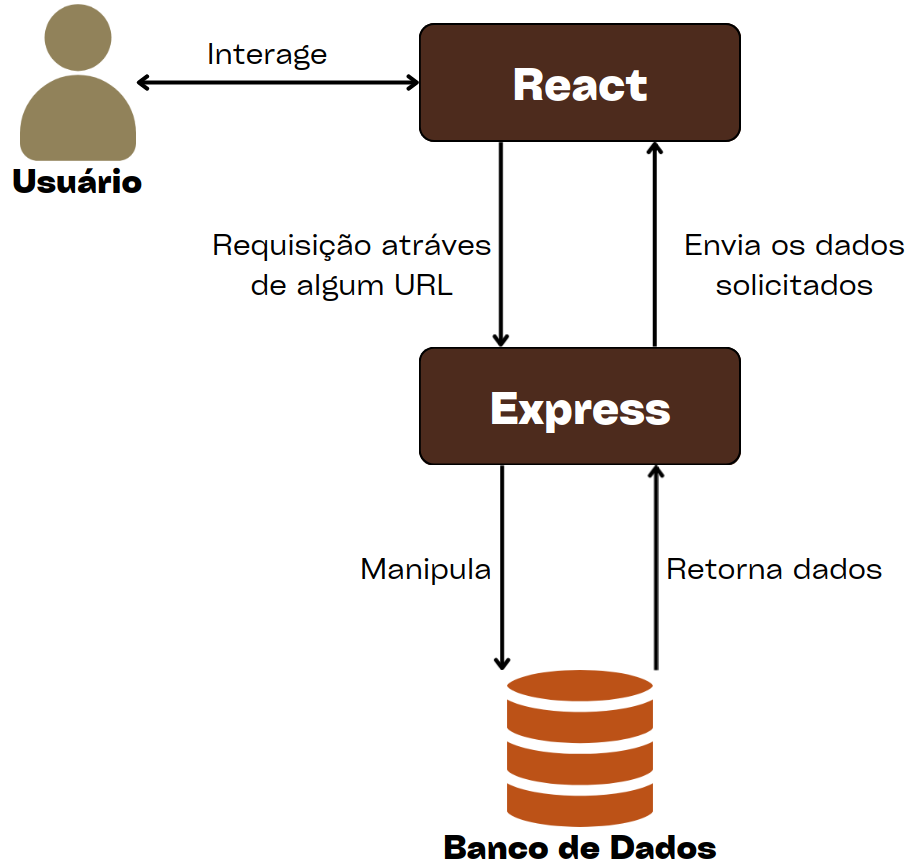
\includegraphics[width=0.5\linewidth]{imagens/architecture.png}
\caption{Arquitetura da aplicação.}
Fonte: própria do autor
\label{fig:architecture}
\end{figure}

\subsubsection{Banco de dados}
O banco de dados foi implementado baseando-se no  diagrama entidade-relacionamento da Figura \ref{fig:er}.

\begin{figure}[hbt!]
\centering
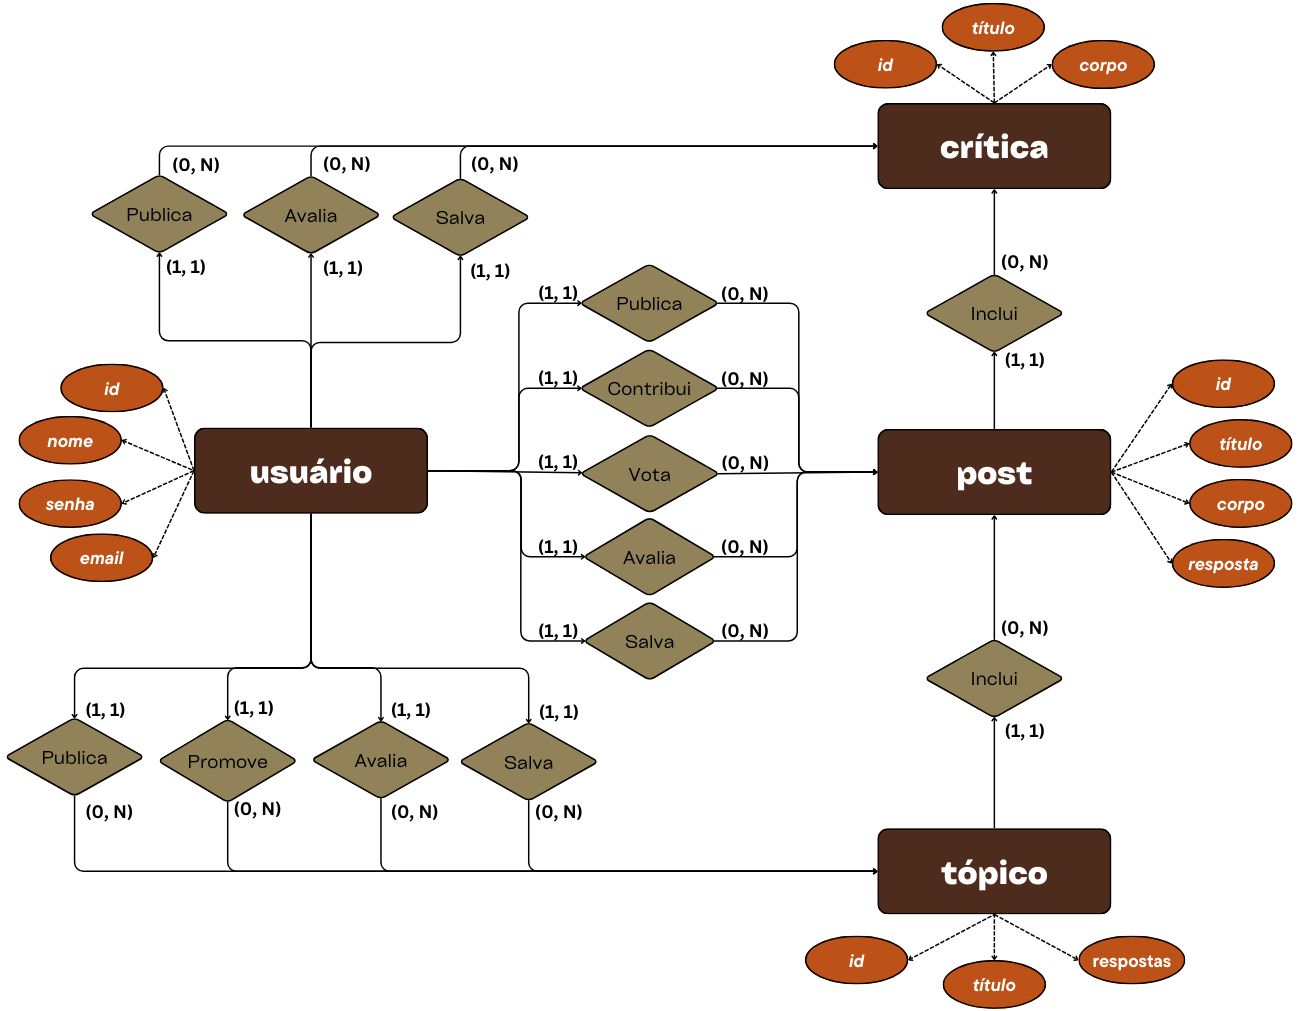
\includegraphics[height=10cm]{imagens/er_diagram.png}
\caption{Diagrama entidade-relacionamento da aplicação.}
Fonte: própria do autor
\label{fig:er}
\end{figure}

As entidades tópico, \textit{post} e crítica foram unificados em uma tabela de conteúdos \textit{contents}, onde a relação entre os conteúdos se dá através de um campo \textit{parent\_id}, que denota o identificador (id) do conteúdo “pai". Para as relações de avaliação, voto, promoção, contribuição e salvamento foram todas consideradas em um tabela de interações \textit{interactions}, na qual o tipo da interação é especificado por uma coluna \textit{type}.

Todos os dados da aplicação foram armazenados utilizando o \textit{PostgreSQL}, com exceção dos dados de corpo dos \textit{posts}, que foram armazenados em arquivos locais gerenciados pelo \textit{Git}, como um SGBD. Cada tópico criado corresponde à uma pasta que contém um repositório \textit{Git}, a partir do qual, para cada \textit{post} criado, cria-se uma nova \textit{branch} correspondente.




\subsection{Interface da aplicação}
A seguir, seguem imagens do design desenvolvido para a aplicação. Como o design depende da existência de conteúdos publicados, fizemos uso de dados \textit{mock}, i.e., dados simulados, para o preenchimento dos campos. Para a paleta de cores utilizada no design da aplicação, foram escolhidas cores visando minimizar a emissão de luz azul, dado que existem evidências que apontam que a luz azul artificial pode prejudicar o sono \cite{blueWorsenSleep}, apesar de que existem outros estudos que ainda apontam inconclusividade em relação a este ponto e outros supostos malefícios da luz azul artificial \cite{blueInconclusive}.


\subsubsection{Principais componentes}
Nesta seção, iremos especificar os principais componentes implementados para compor a interface da aplicação.

\paragraph{\textit{Frame}}

Um \textit{frame}, ou quadro (Figura \ref{fig:frame}), é uma unidade básica de composição, em que outros componentes serão montados em cima. Ele fornece:
\begin{itemize}
    \item \textbf{Botões de voto e avaliação}: São compostos pelas setas e o círculo antes do título, as setas correspondem aos botões de avaliação de relevância, com a seta para cima indicando um conteúdo relevante e, para baixo, um conteúdo não relevante. O botão de voto pode ser usado para múltiplas finalidades que serão descritas nas seções dos próximos componentes;
    \item \textbf{Campo de botões utilitários}: Representado pelos três pontos no canto superior direito, podem ser fornecidos botões com texto e ícones que realizam alguma função quando clicados. Vale ressaltar que no design para \textit{desktop} os ícones são mostrados diretamente, enquanto para \textit{mobile} somente são visíveis ao clicar no ícone de três pontos, abrindo um menu;
    \item \textbf{Campo de corpo}: Pode ser texto ou outros componentes;
    \item \textbf{Campo de rodapé}: Pode ter texto ou uma lista de itens;
    \item \textbf{Campo de título}.
\end{itemize}


\begin{figure}[hbt!]
\centering
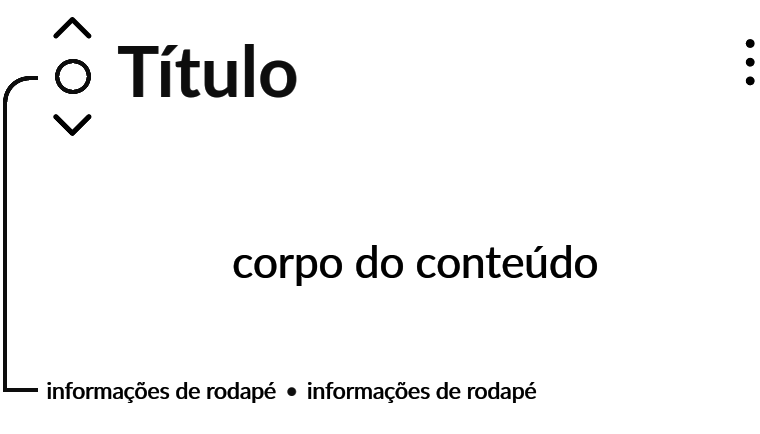
\includegraphics[width=0.5\linewidth]{imagens/structure/frame.png}
\caption{Estrutura do \textit{frame}.}
Fonte: própria do autor
\label{fig:frame}
\end{figure}


\paragraph{Tópico}

O tópico contém os seus \textit{posts} de resposta dispostos em ordem decrescente de votos. Os \textit{posts} de cada tópico são expostos em duas partes (Figura \ref{fig:topic}): uma barra com o título do \textit{post} de tamanho proporcional à sua porcentagem de votos e os primeiros 280 caracteres do texto do \textit{post}. \textit{Posts} escritos pelo usuário tem um símbolo de um lápis antes de seu título, e o \textit{post} votado pelo usuário contém um símbolo de uma estrela e uma cor de fundo diferente para a barra. O usuário pode promover o tópico ao clicar no botão de voto, além disso, pode salvar o tópico ao clicar no símbolo de \textit{bookmark} e responder o tópico criando um \textit{post}, ao clicar na seta apontada para esquerda.

\begin{figure}[hbt!]
\centering
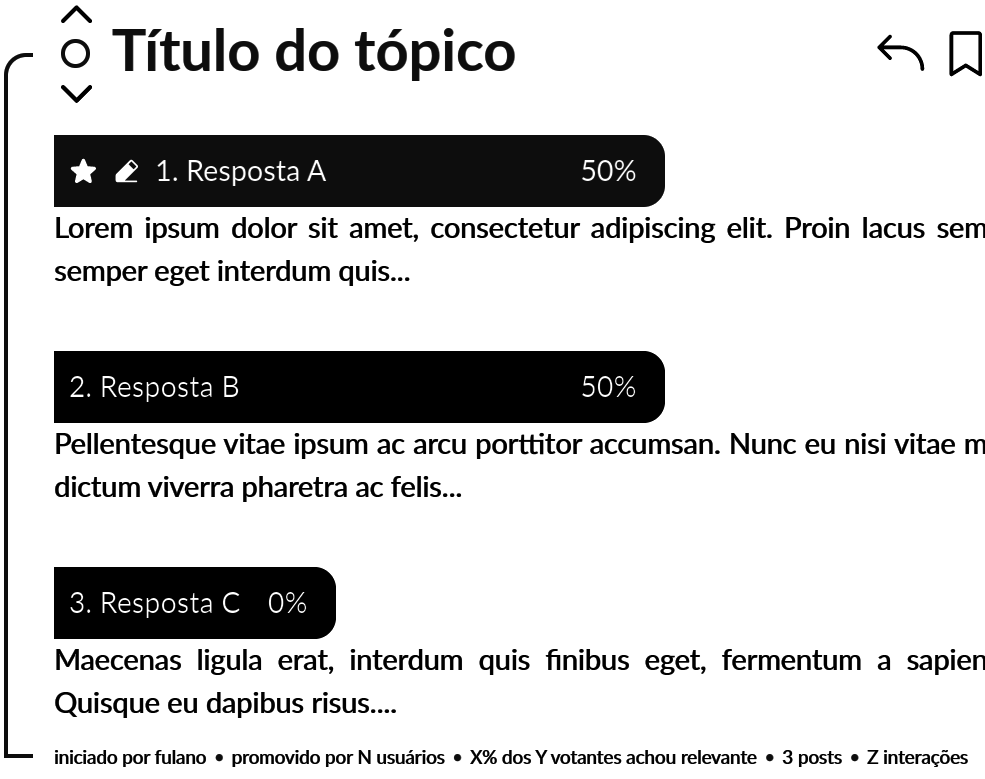
\includegraphics[width=0.7\linewidth]{imagens/structure/topic.png}
\caption{Estrutura do tópico.}
Fonte: própria do autor
\label{fig:topic}
\end{figure}



\paragraph{\textit{Post}}

O \textit{post} pode ter, como parte de seu corpo, texto, com as principais funcionalidades de formatação do \textit{Markdown}, além de gráficos e tabelas. O seu botão de voto se destina a realizar o voto no \textit{post corrente} como resposta ao tópico, já os botões utilitários têm as seguintes funções, seguindo da esquerda para a direita:
\begin{itemize}
    \item \textbf{Criar uma \textit{branch}}: Atende ao [RF14], somente visível para usuários que não sejam o autor do post;
    \item \textbf{Realizar \textit{merge} de uma \textit{branch}}: Atende ao [RF17], somente visível para o autor do \textit{post}. Há um contador indicando quantas sugestões foram recebidas;
    \item \textbf{Ocultar/expor críticas};
    \item \textbf{Editar o conteúdo do \textit{post}}: Permite o usuário editar o conteúdo do \textit{post}, quando o usuário terminar, ele pode clicar novamente no ícone e então uma caixa de diálogo será aberta para que ele escolha o que fazer com suas edições. Caso seja o autor, atualiza diretamente o \textit{post}, atendendo ao [RF12], caso não, cria uma nova sugestão de \textit{post}, atendendo ao [RF13];
    \item \textbf{Salvar o \textit{post}}.
\end{itemize}

\begin{figure}[hbt!]
\centering
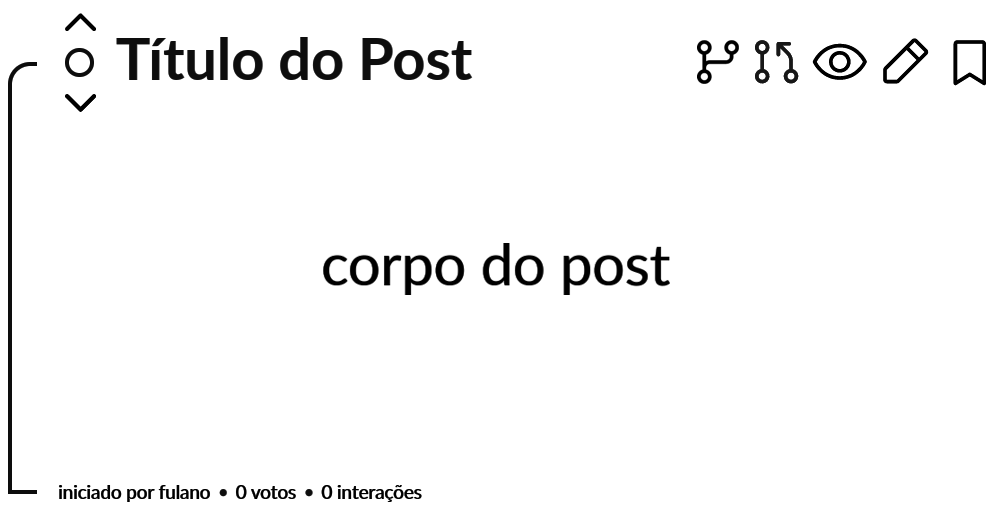
\includegraphics[width=0.7\linewidth]{imagens/structure/post.png}
\caption{Estrutura do post.}
Fonte: própria do autor
\label{fig:post}
\end{figure}



\paragraph{Crítica}

A crítica não contém um botão de voto, e só tem um botão para salvá-la e um botão para fechá-la. Em seu rodapé consta o nome do autor e a quantidade e divisão dos votos de avaliação de relevância.


\subsubsection{Páginas}

\paragraph{Página de árvore de tópicos}

A tela de visualização de tópicos (Figura \ref{fig:topicTree}) é a tela principal da aplicação e contém até 5 tópicos, sendo o restante acessível por meio do uso de um componente de paginação. Cada tópico exibe os 3 \textit{posts} mais votados, podendo o restante ser visualizado ao entrar na página do tópico através de um clique no título do tópico, ou em reticências que aparecem em seu canto inferior, caso hajam mais de 3 \textit{posts}. Por fim, o conteúdo pode ser ordenado por número de promoções, na aba “promovido" e por ordem de criação, na aba “todos".
\begin{figure}[hbt!]
\centering
\begin{subfigure}{.3\textwidth}
  \centering
  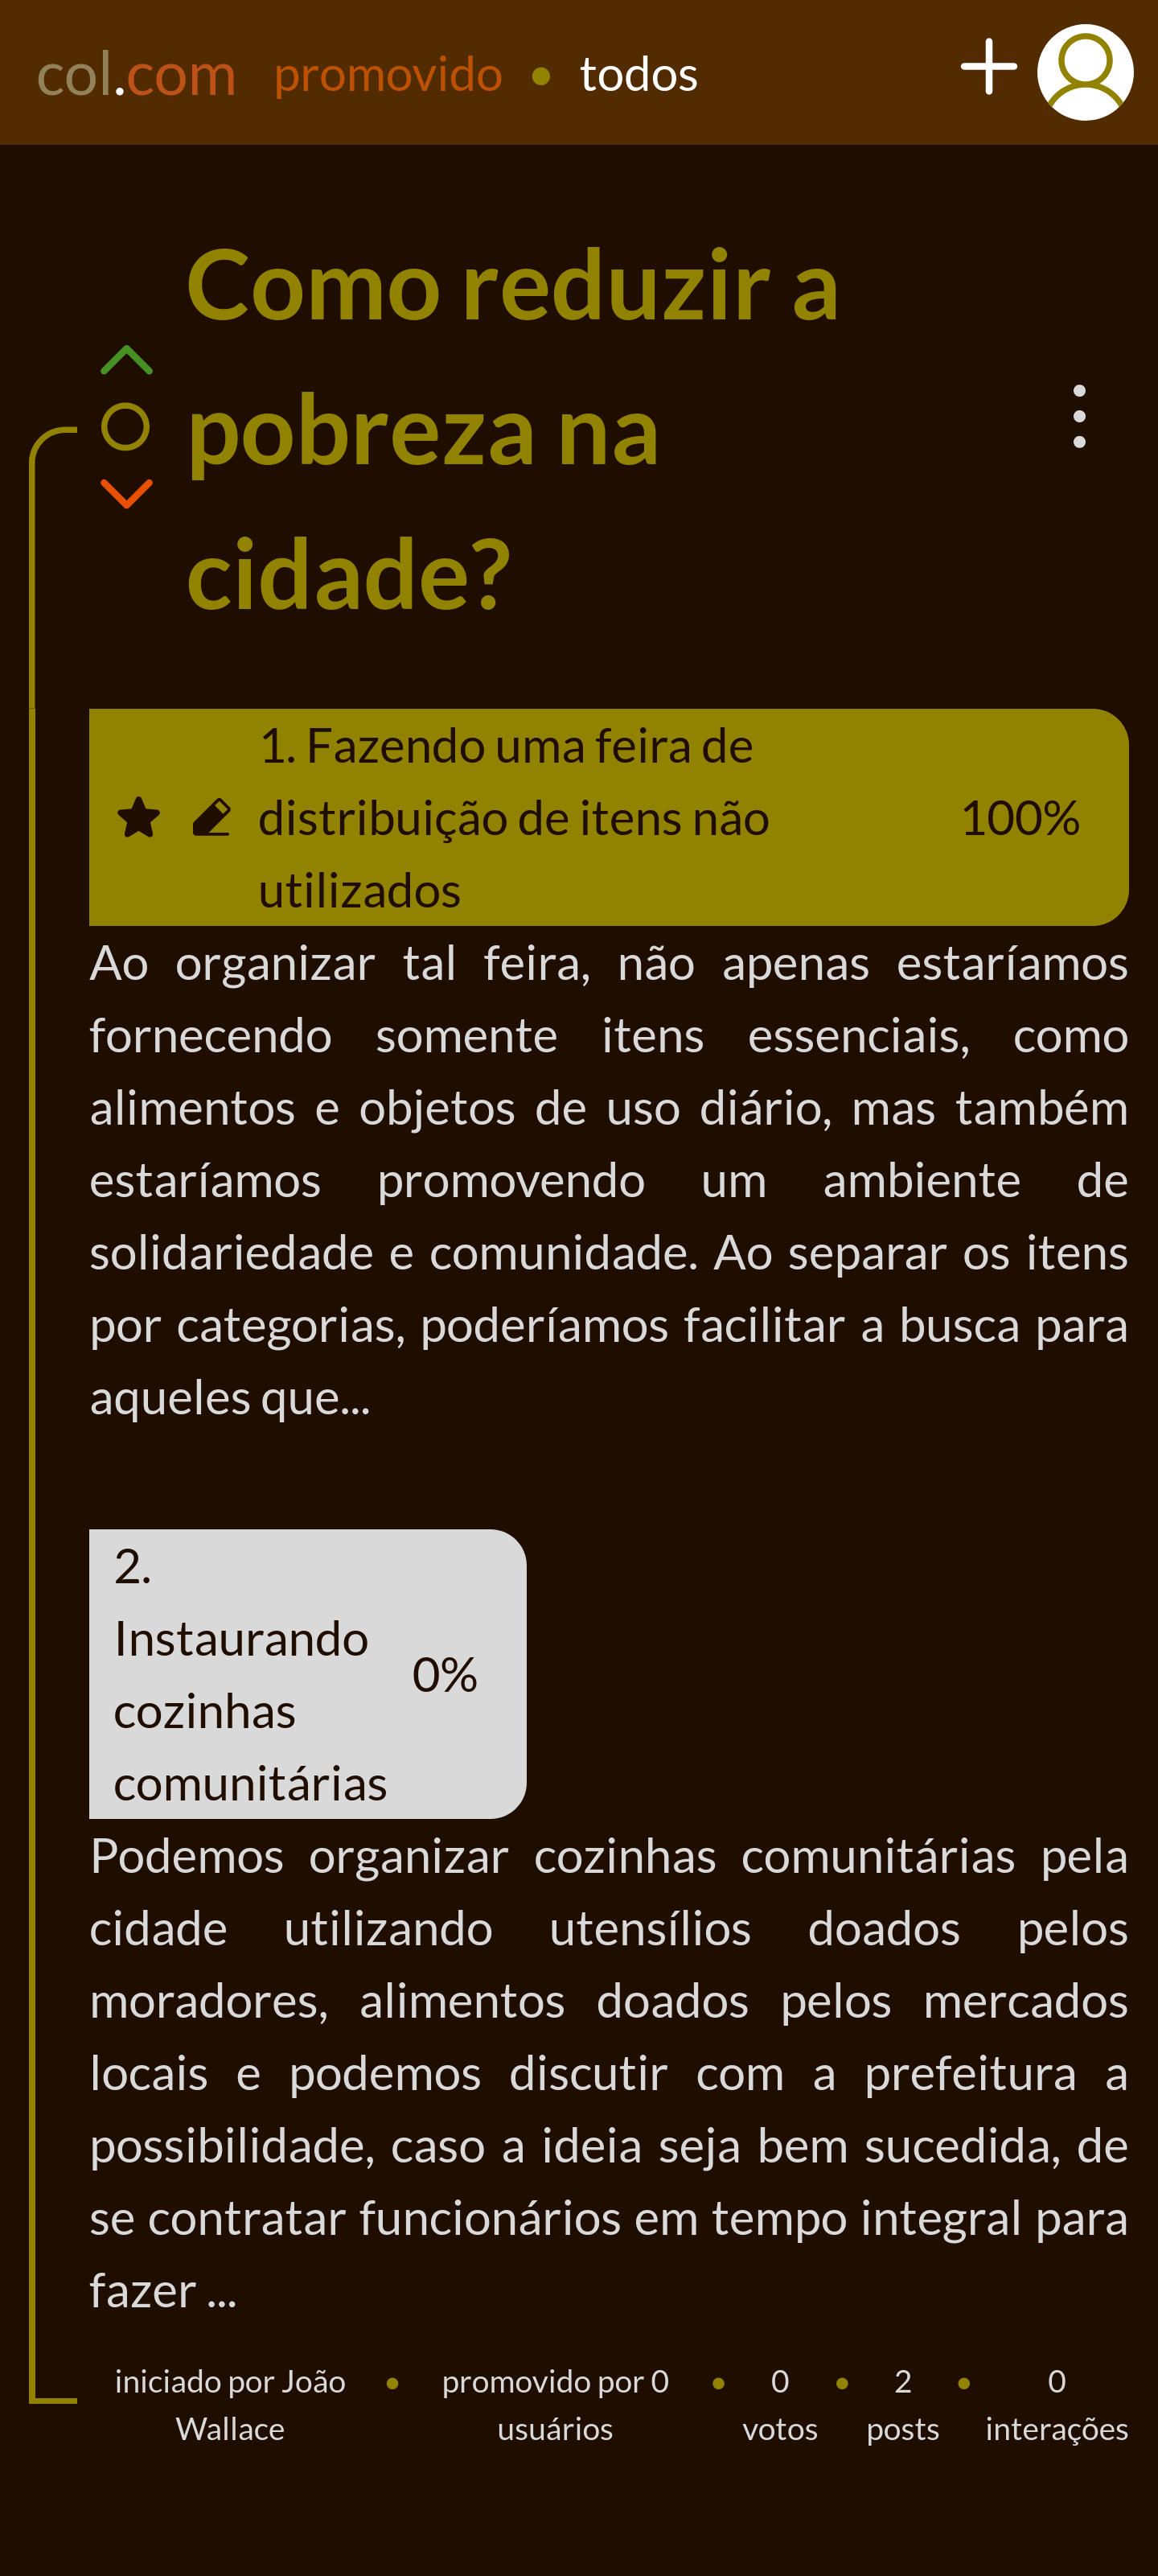
\includegraphics[width=.7\linewidth]{imagens/captures/m_topics.png}
  \caption{Versão mobile}
\end{subfigure}%
\begin{subfigure}{.7\textwidth}
  \centering
  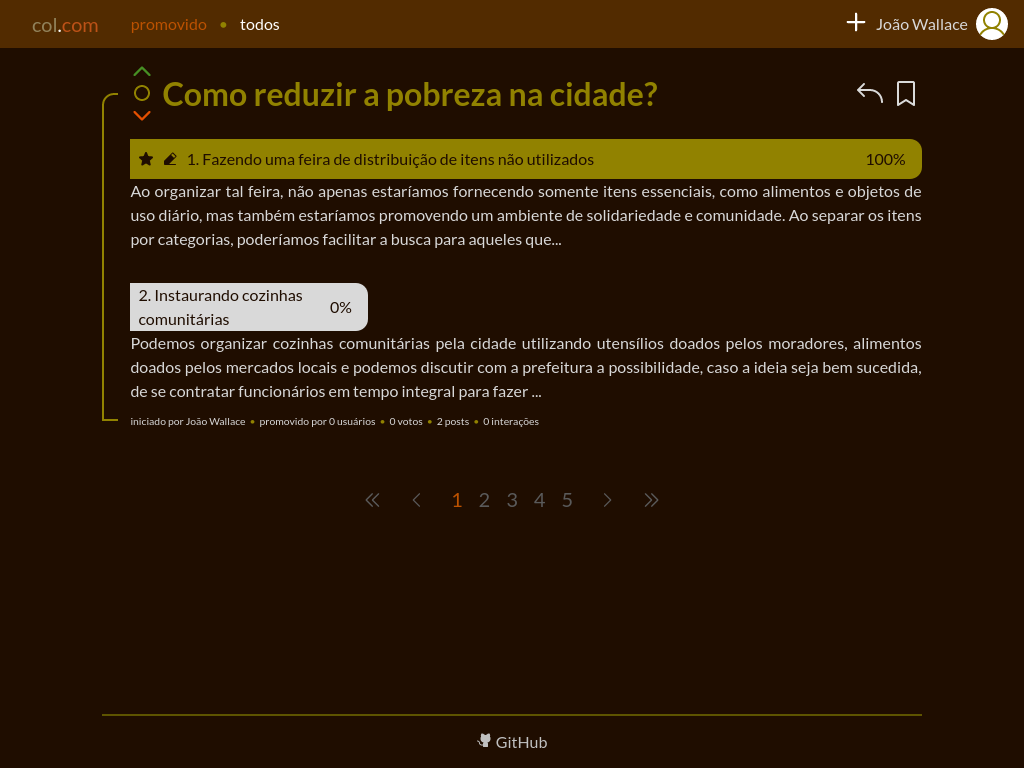
\includegraphics[width=0.9\linewidth]{imagens/captures/topics.png}
  \caption{Versão \textit{desktop}}
\end{subfigure}
\caption{Tela de visualização dos tópicos.}
\label{fig:topicTree}
\end{figure}



\paragraph{Página de tópico}
A página de tópico é semelhante à página de árvore de tópicos, entretanto, só contém um componente de tópico e todos os seus \textit{posts} associados.

% \newpage

\paragraph{Página de \textit{post}}

Como exposto na Figura \ref{fig:postPage}, a tela de um \textit{post} é composta por três elementos, sendo eles de cima para baixo: um \textit{link} para seu tópico pai, uma barra \textit{slider}, para seleção da versão e o \textit{post} em si. Através da tela de \textit{post}, também é possível visualizar as críticas realizadas ao \textit{post} em cada uma de suas versões, como demonstrado na Figura \ref{fig:postCritique}. Críticas feitas em trechos que se sobrepõem são unidas em um mesmo bloco que, ao ser clicado, exibe a lista de todas as críticas contidas nele; para se identificar o trecho específico de uma crítica contida em um bloco, o usuário pode clicar em seu título, assim marcando o trecho condizente.


\begin{figure}[hbt!]
\centering
\begin{subfigure}{.3\textwidth}
  \centering
  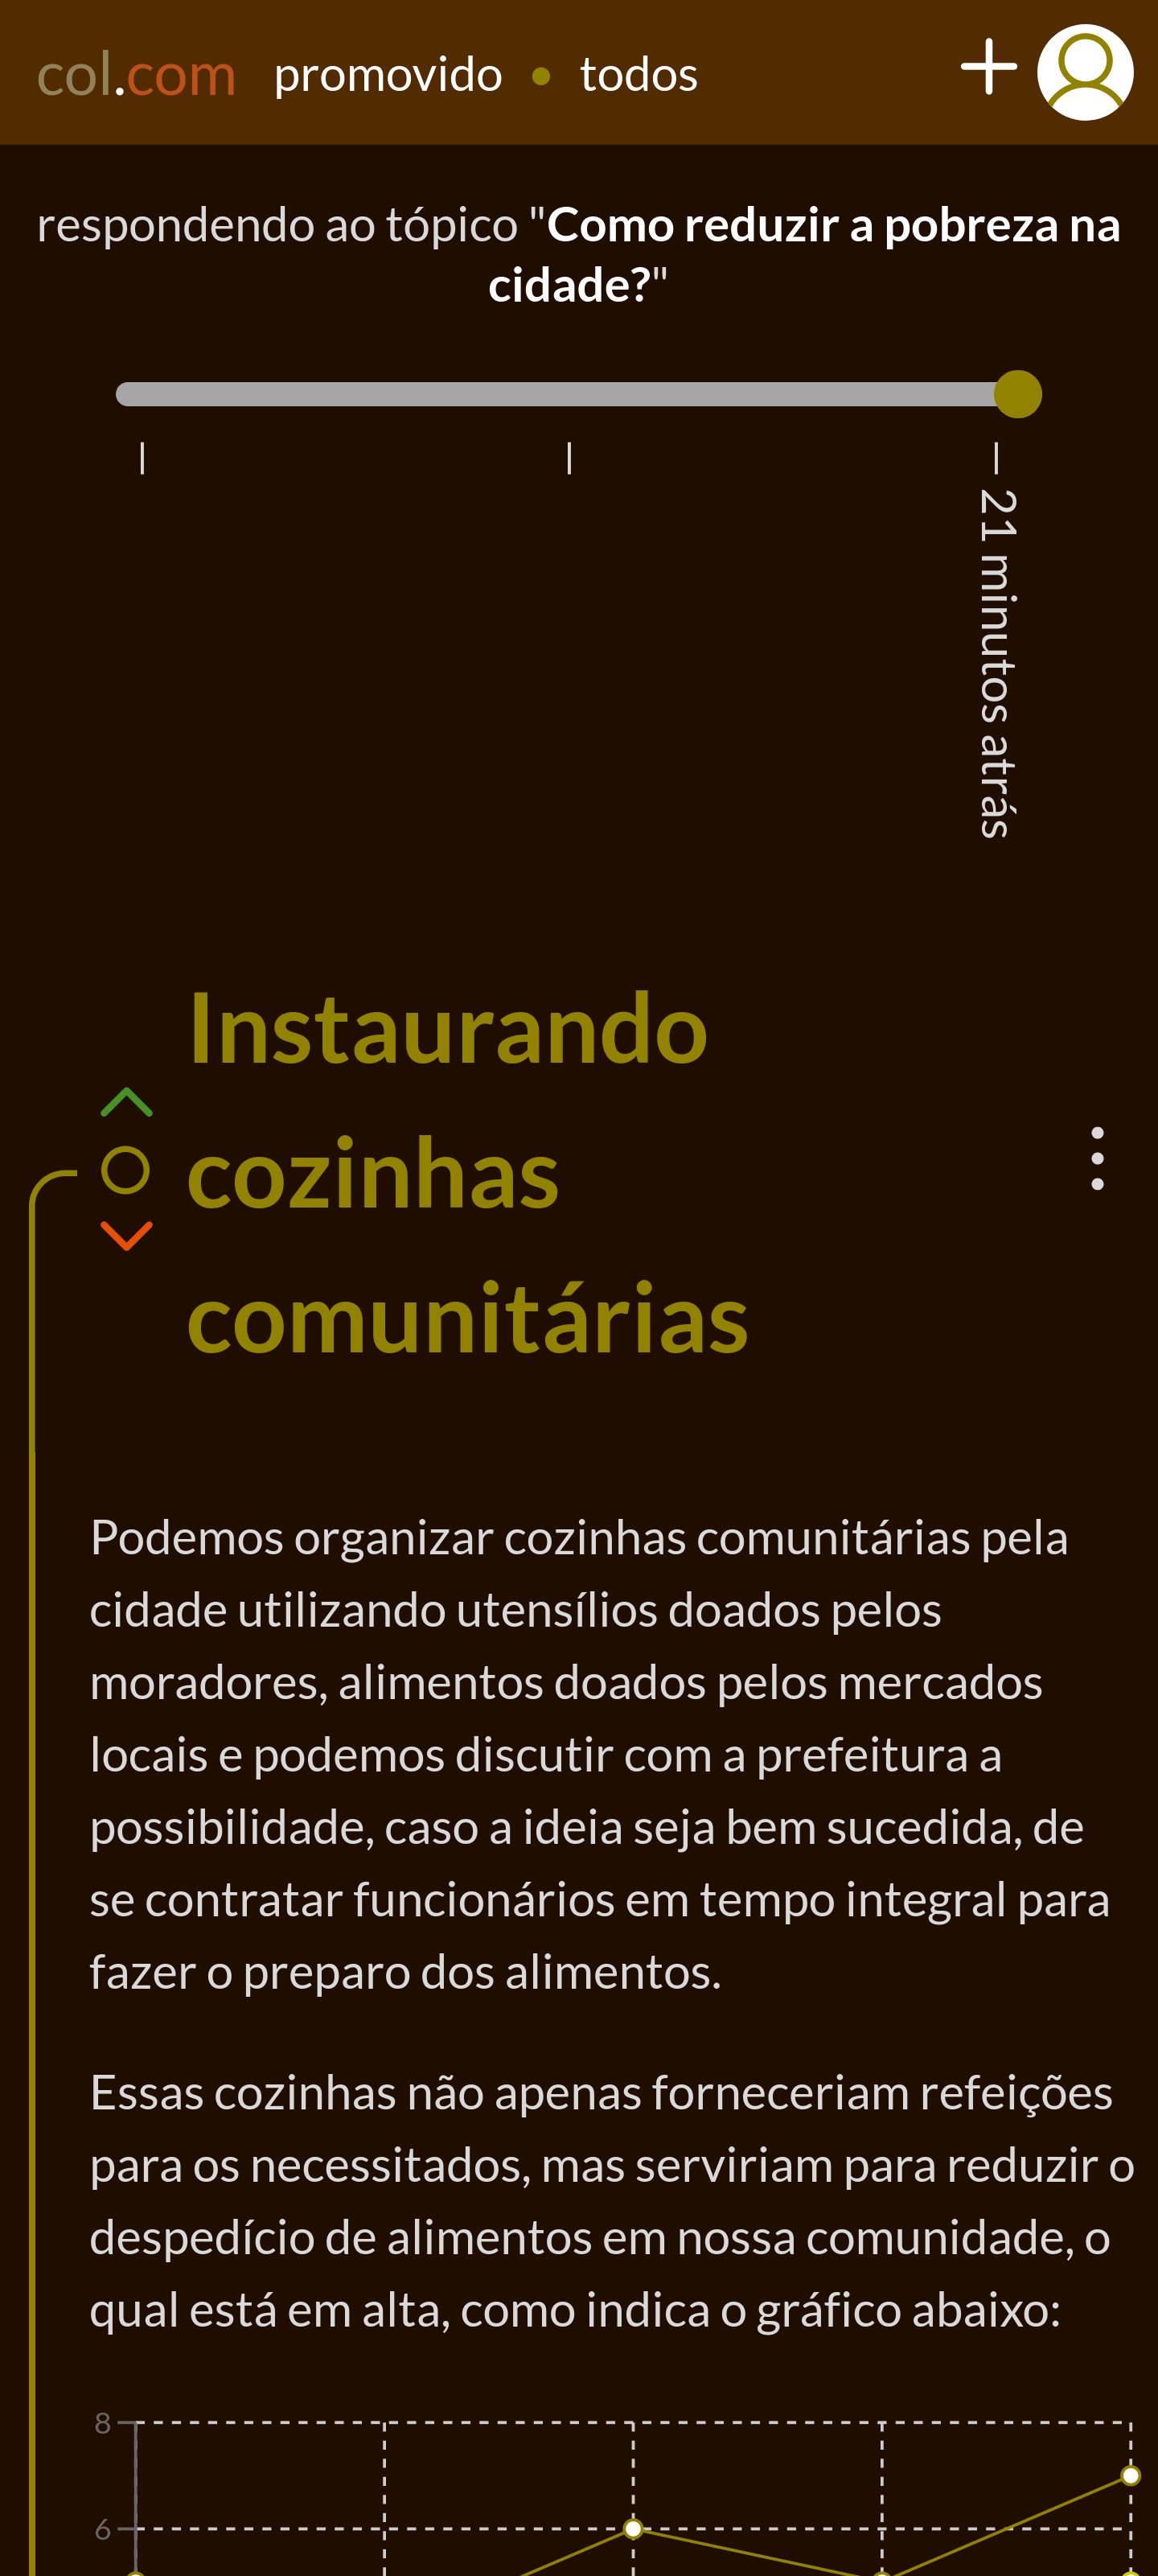
\includegraphics[width=.68\linewidth]{imagens/captures/m_post.png}
  \caption{Versão mobile}
\end{subfigure}%
\begin{subfigure}{.7\textwidth}
  \centering
  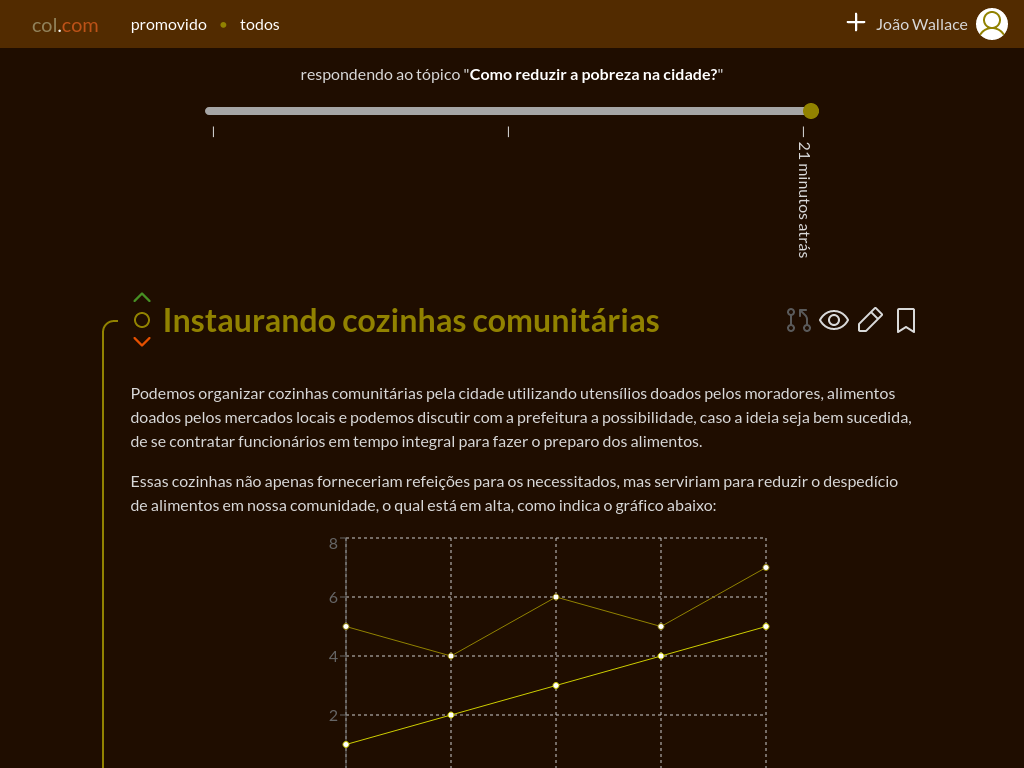
\includegraphics[width=0.87\linewidth]{imagens/captures/post.png}
  \caption{Versão desktop}
\end{subfigure}
\caption{Tela de visualização do \textit{post}.}
\label{fig:postPage}
\end{figure}


\begin{figure}[hbt!]
\centering
\begin{subfigure}{.3\textwidth}
  \centering
  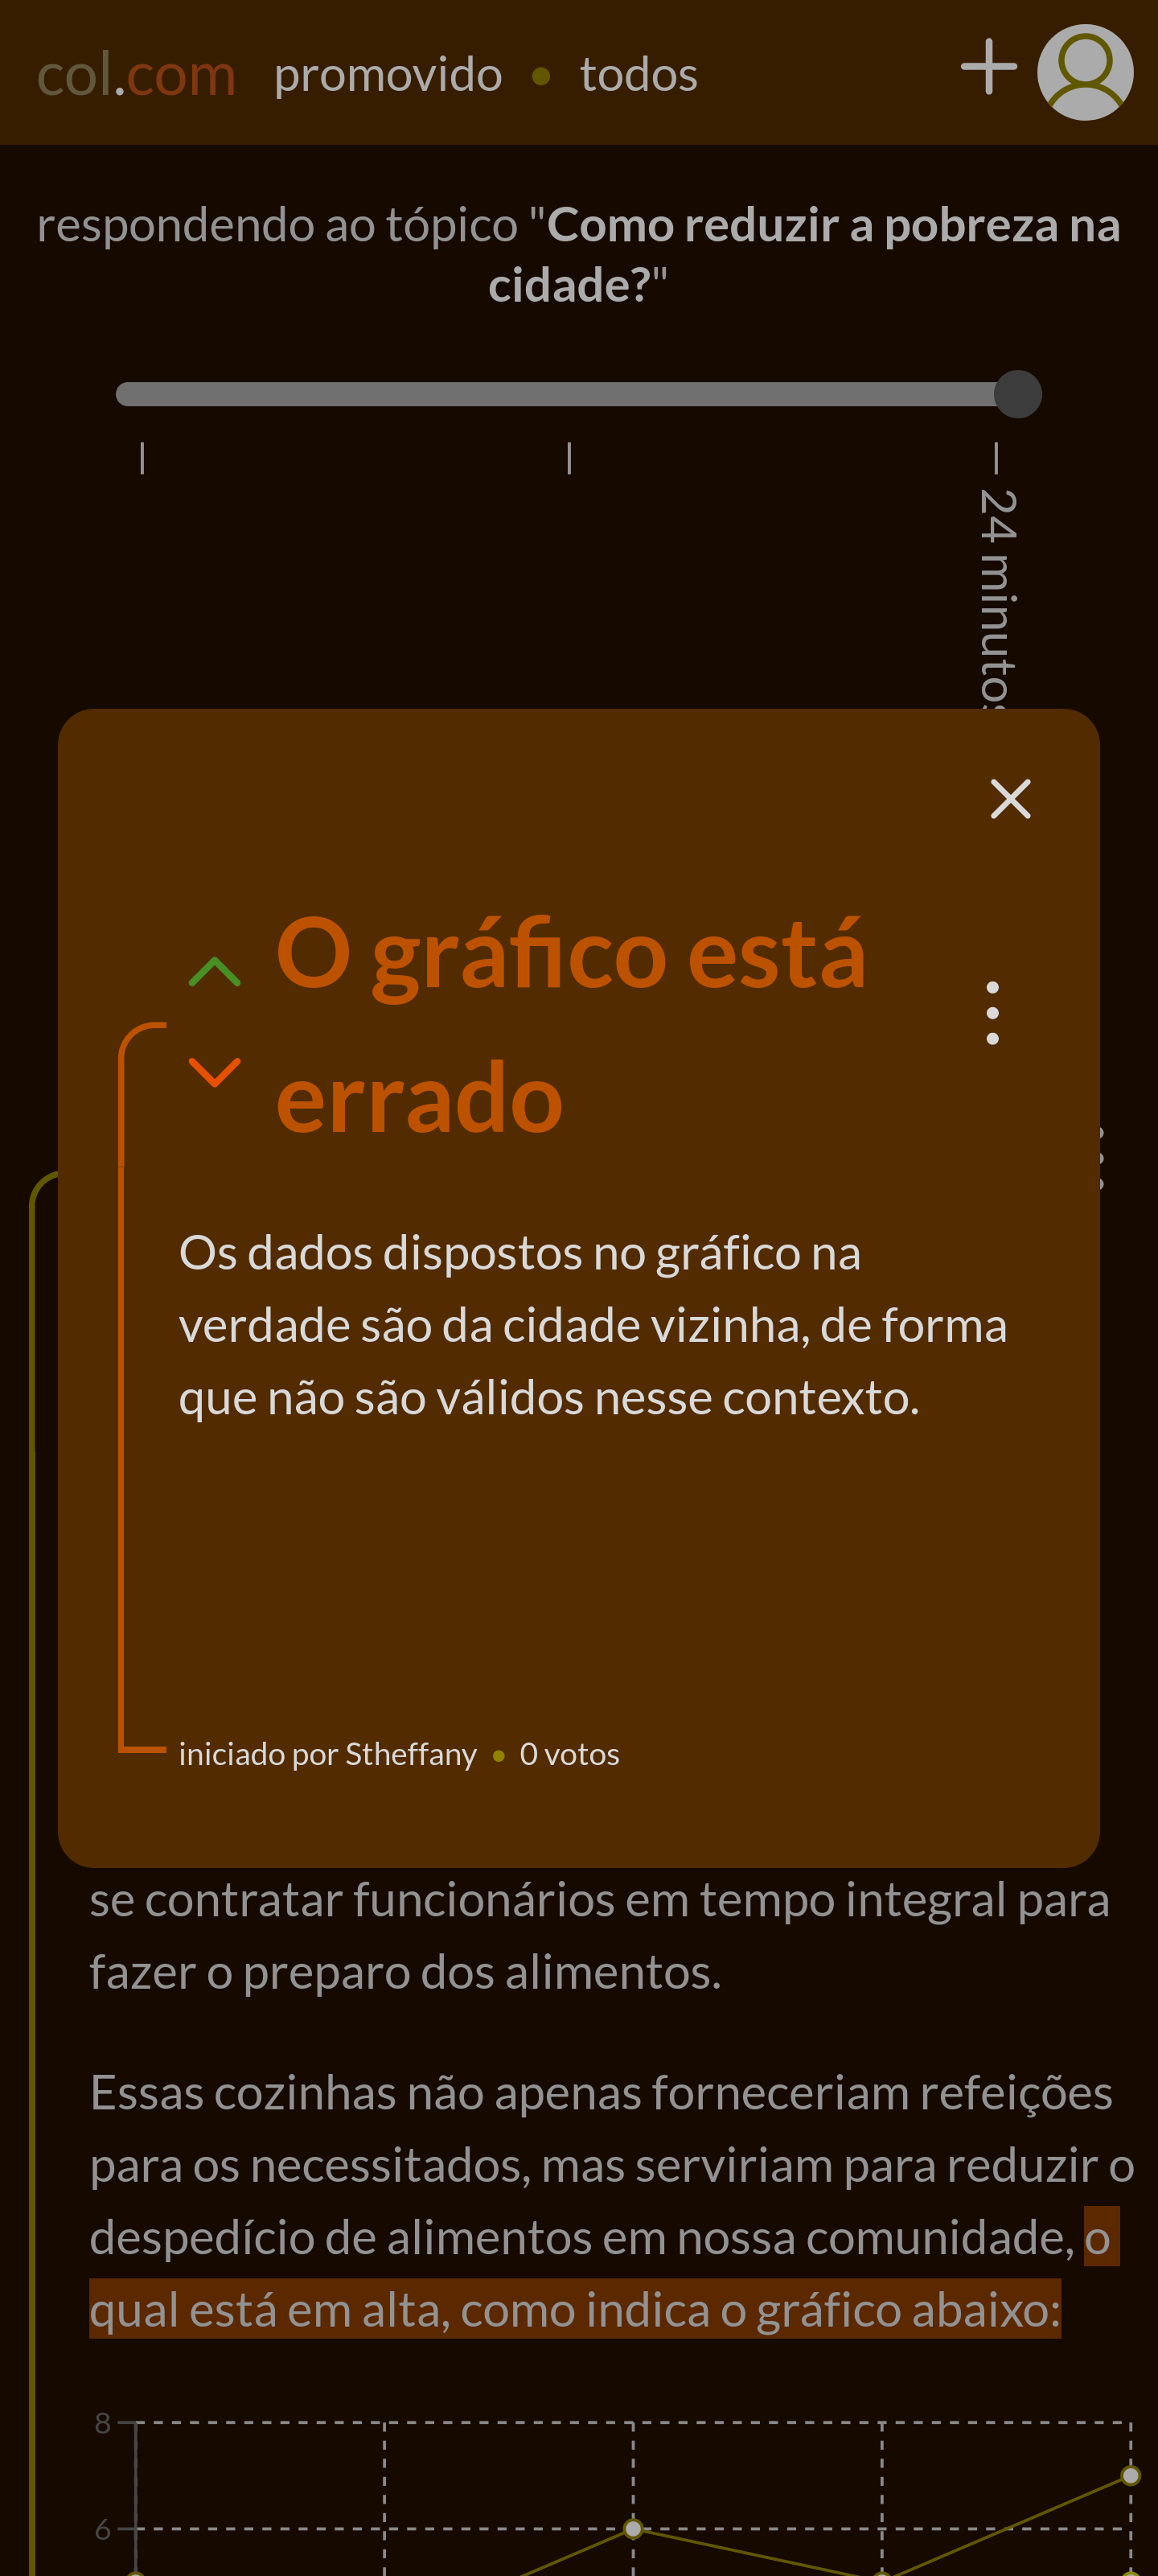
\includegraphics[width=.68\linewidth]{imagens/captures/m_post_critique.png}
  \caption{Versão mobile}
\end{subfigure}%
\begin{subfigure}{.7\textwidth}
  \centering
  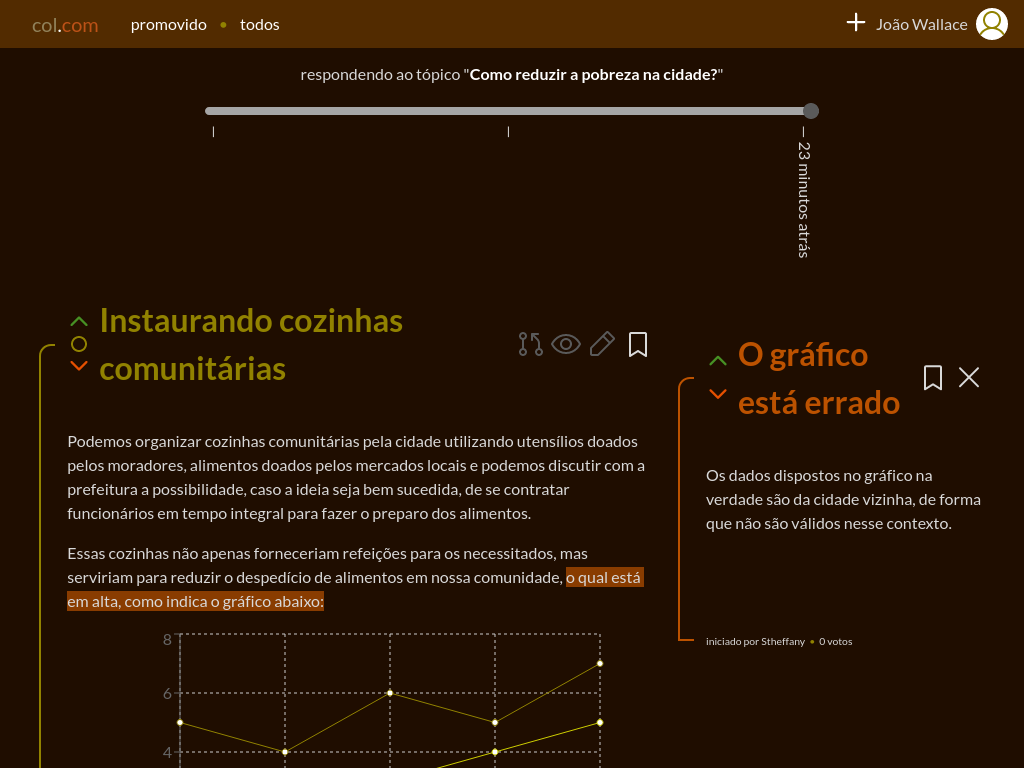
\includegraphics[width=0.87\linewidth]{imagens/captures/post_critique.png}
  \caption{Versão desktop}
\end{subfigure}
\caption{Tela de um post com uma crítica sendo visualizada.}
\label{fig:postCritique}
\end{figure}


\paragraph{Página de \textit{login} e cadastro}
O \textit{login} e cadastro do usuário são realizados na mesma página, esta exposta na Figura \ref{fig:login}, sendo possível alternar entre duas operações ao clicar no texto “crie uma agora!", para se direcionar ao cadastro, e “entre agora!" para o \textit{login}. O formulário de cadastro é exposto na Figura \ref{fig:signup}.

\begin{figure}[hbt!]
\centering
\begin{subfigure}{.3\textwidth}
  \centering
  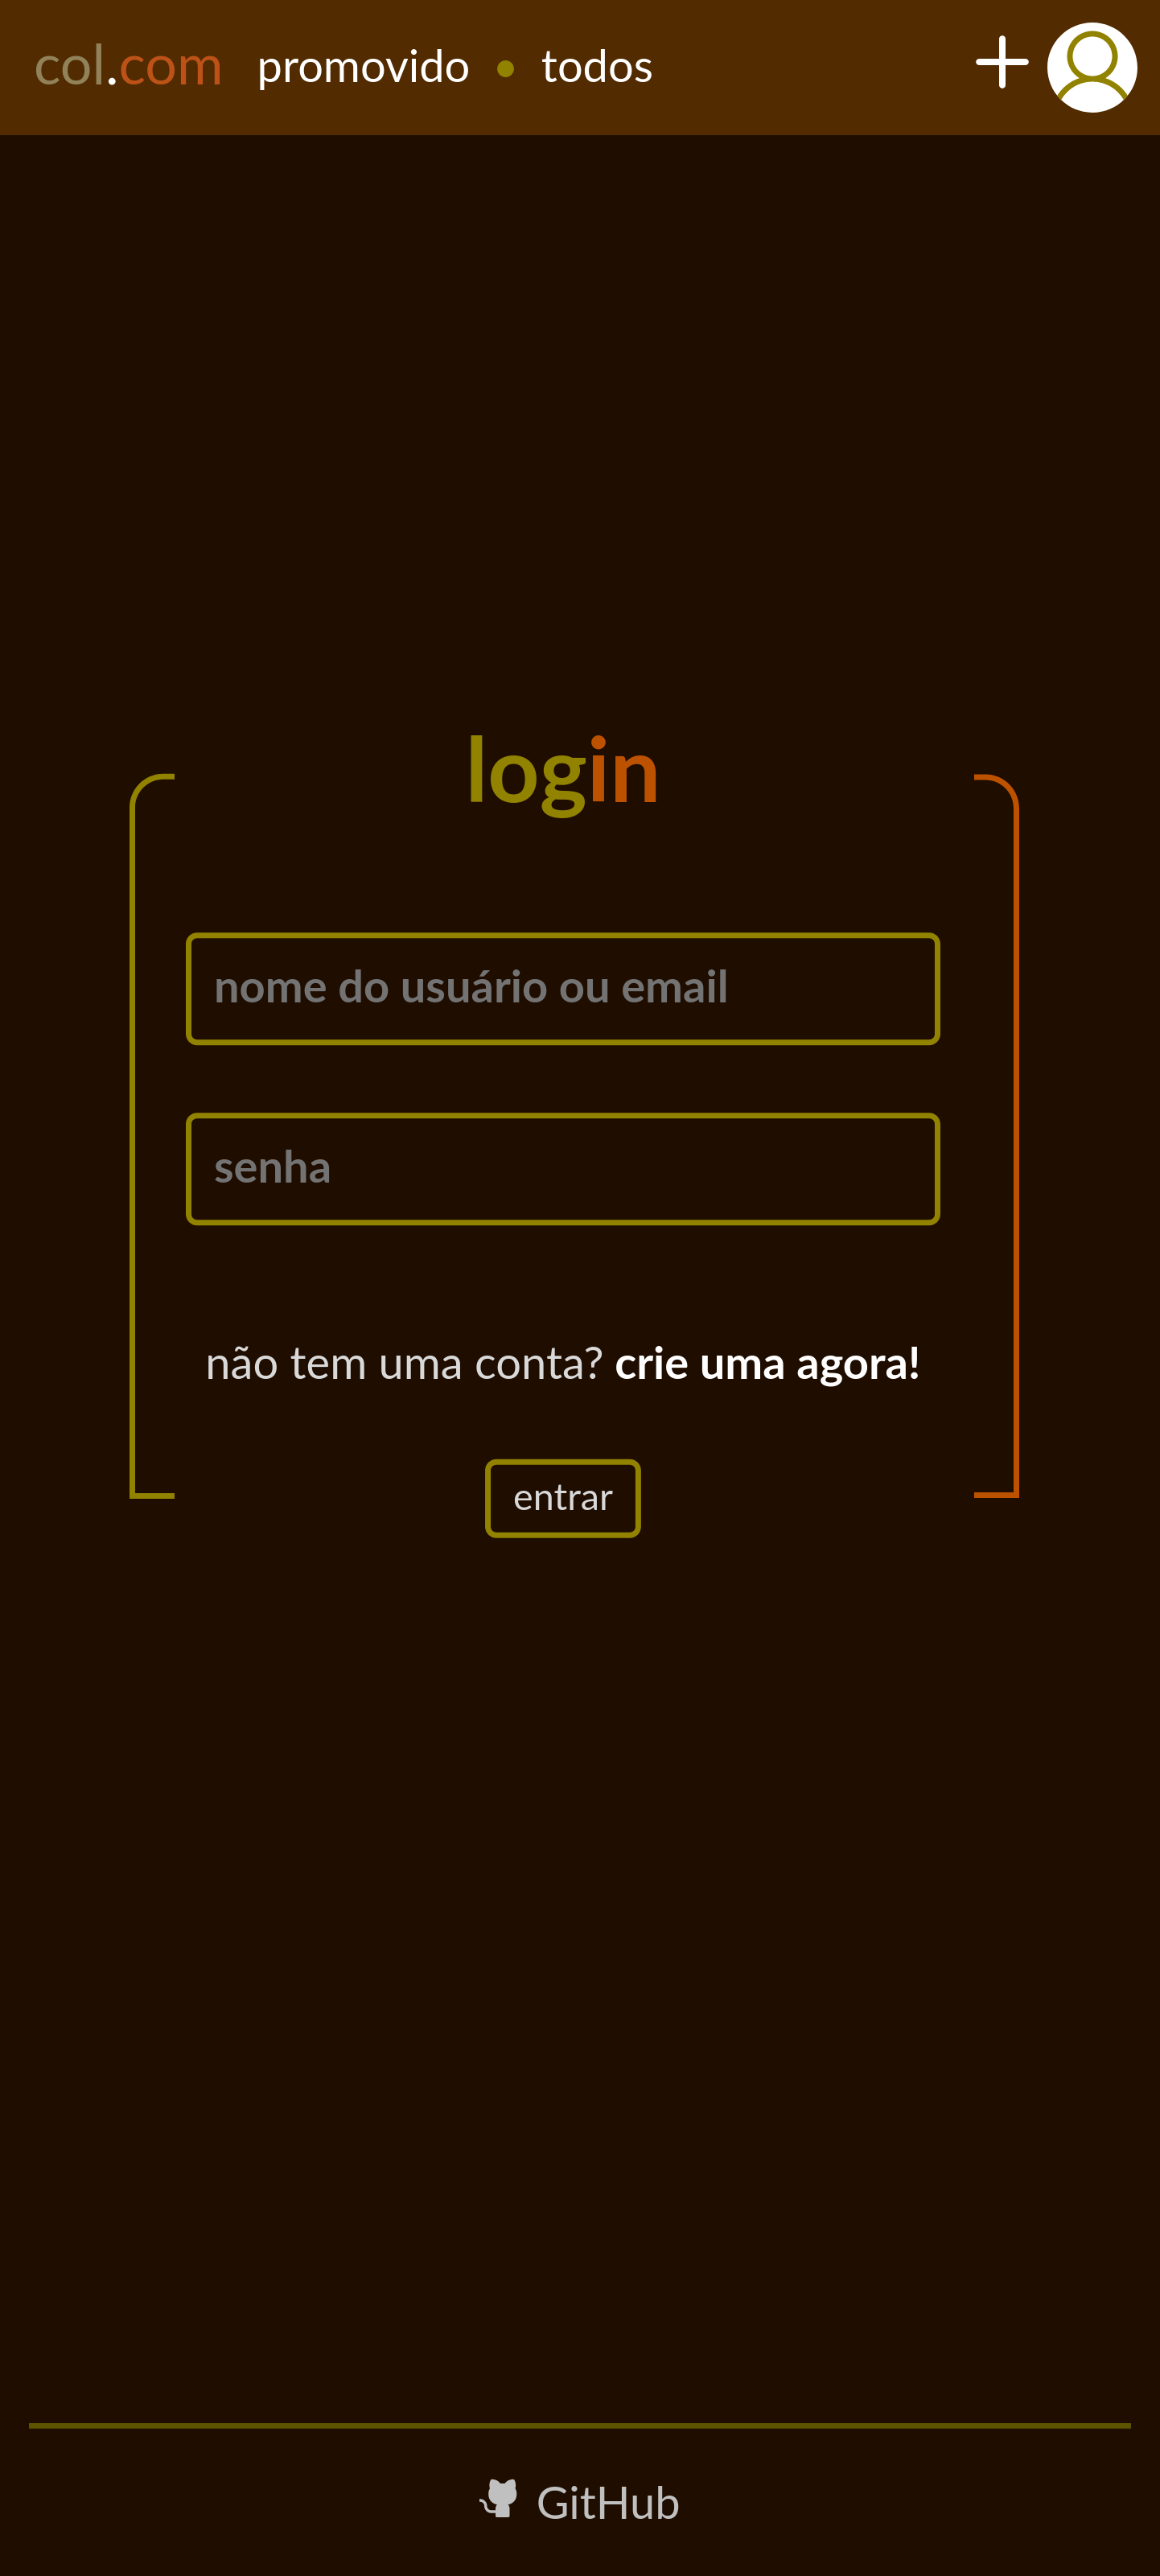
\includegraphics[width=.66\linewidth]{imagens/captures/m_login.png}
  \caption{Versão mobile}
\end{subfigure}%
\begin{subfigure}{.7\textwidth}
  \centering
  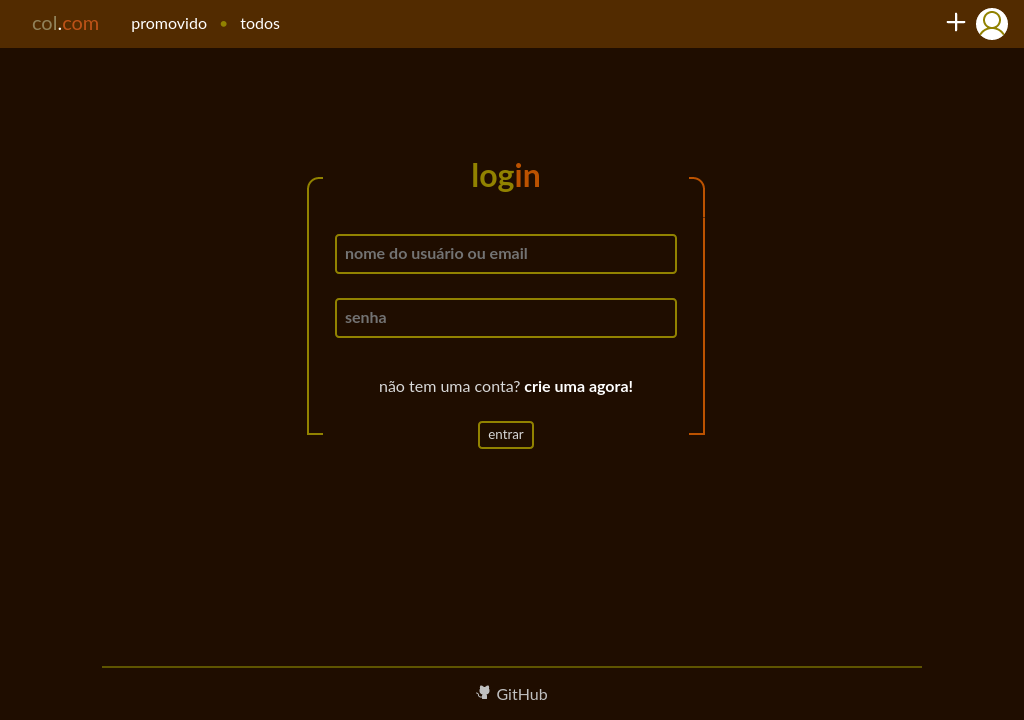
\includegraphics[width=0.9\linewidth]{imagens/captures/login.png}
  \caption{Versão desktop}
\end{subfigure}
\caption{Tela de \textit{login} e cadastro.}
\label{fig:login}
\end{figure}

\begin{figure}[hbt!]
\centering
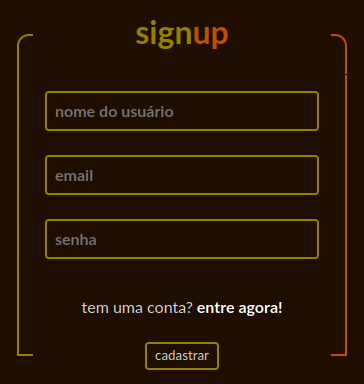
\includegraphics[width=0.275\linewidth]{imagens/captures/signup.png}
\caption{Formulário de cadastro.}
\label{fig:signup}
\end{figure}

\paragraph{Página de conteúdos salvos}
A página de conteúdos salvos contém todos os tópicos, \textit{posts} e críticas salvos pelo usuário, dispostos de maneira similar à árvore de tópicos.

\paragraph{Página de edição de texto}
Na página de edição de texto, o usuário pode escrever um \textit{post}, informando um título e fornecendo um corpo. O corpo do \textit{post} pode conter texto, com estilizações do \textit{Markdown}, tabelas e gráficos.

\clearpage